p% !TEX encoding = UTF-8 Unicode
\documentclass{article}


\usepackage[square]{natbib}


\usepackage[spanish,es-nodecimaldot]{babel}		
\usepackage[utf8]{inputenc}
\usepackage[T1]{fontenc}
 \usepackage[pdftex]{graphicx}	
 \usepackage{wrapfig}	
%\usepackage{afterpage}

%\renewcommand{\rmdefault}{phv}
%\renewcommand{\sfdefault}{phv}


\usepackage{amsmath,amsfonts,amsthm,amssymb} % Math packages
% Table/figure positioning
\usepackage{float}
\restylefloat{table}





		
\title{Modelos Bayesianos Jerárquicos}
\author{\Large José Luis Baroja
\thanks{Financiado por el proyecto PAPIIT \bf{IN307214}}
	\\\emph{Facultad de Psicología, UNAM}
	}
	
\date{}


%\newcommand{\Mzero}{$\mathcal M_{0}$}


\begin{document}
\maketitle
%\begin{abstract}
%Resumen pendiente...
%\end{abstract}

Supón que a lo largo del semestre registramos el número de canciones que cierta persona baila en diferentes fiestas. Al final del curso el registro puede verse así:\\

\centerline{ $c$ : \texttt{\;\;5\;\;\;\;3\;\;\;\;4\;\;\;\;7\;\;\;\;4\;\;\;\;5\;\;\;\;5\;\;\;\;4\;\;\;\;5\;\;\;\;7\;\;\;\;7\;\;\;\;6}}\hfill

\noindent en donde cada posición $c_f$ del vector $c$ corresponde con el número de canciones que la persona bailó en la fiesta $f$.\\
\indent Supón también que estamos interesados en utilizar los datos que recolectamos para averiguar qué tanto le gusta bailar a la persona en observación. Una aproximación que permite utilizar las observaciones registradas para aprender sobre nuestro sujeto consiste en construir un modelo que especifica cómo se relaciona el rasgo \emph{gusto por bailar} con el número de canciones que la persona bailó en cada fiesta  del semestre.\\
\indent En este capítulo mostraremos cómo podemos construir dicho modelo y cómo podemos extenderlo para aprender no sólo sobre una persona sino también sobre poblaciones de individuos. La aproximación y modelos que presentamos pueden utilizarse para aprender sobre un amplio conjunto de características psicológicas en diferentes poblaciones de organismos.\\ 
\indent El plan del capítulo es el siguiente: primero construiremos un modelo para inferir el gusto por bailar de nuestra primera persona. Después mostraremos cómo podemos extender este modelo para aprender sobre varias personas. Posteriormente ampliaremos el modelo para varias personas de tal manera que también nos permita llegar a conclusiones sobre la población de la que las personas forman parte. Finalmente presentaremos una extensión adicional que permite aprender al mismo tiempo no sólo sobre cada persona y sobre la población de personas, sino también sobre cada fiesta y sobre la población de fiestas.\\\\
\indent Para inferir el gusto por bailar de la primera persona comenzaremos con un supuesto central: Asumiremos que la probabilidad de bailar cierto número de canciones $c_f$ es una función de cierto valor $\lambda$ que representa el \emph{gusto por bailar} de la persona. Nuestro modelo debe capturar la intuición de que si una persona tiene una valor $\lambda$ alto es altamente probable que baile muchas canciones. Por el contrario, si la persona tiene un valor $\lambda$ bajo entonces deberíamos esperar que baile pocas canciones por fiesta. Una función que cumple estas características es la distribución Poisson. Esta distribución está construida para modelar conteos de eventos que ocurren con cierta tasa a lo largo del tiempo: si sabemos que los taxis pasan aproximadamente cada minuto y medio en cierta calle, la distribución Poisson especifica qué tan problable es observar 0, 1, 2, o cada posible número de taxis en cierto intervalo de tiempo. Intuitivamente, entre menor sea la tasa de ocurrencia del evento, menor es el número esperado de ocurrencias. La Figura \ref{fig:Poisson} ilustra cómo se comporta esta distribución. Cada curva en la Figura \ref{fig:Poisson} representa a una persona con un valor $\lambda$ particular. A la primera persona le gusta bailar poco, lo cual representamos con un valor $\lambda=2$. Dado que la persona tiene un valor $\lambda$ pequeño es altamente probable que baile pocas canciones y poco probable que baile muchas, como lo indica la curva que une los puntos blancos. La segunda persona, representada por la curva de puntos grises, tiene un valor de $\lambda=5$. Como consecuencia, es altamente probable que esta persona baile entre 3 y 6 canciones por fiesta y poco probable que baile más de 8 o 9. La última persona tiene un valor $\lambda=10$. Los puntos negros, que representan la distribución Poisson asociada a este valor $\lambda$, muestran que es altamente probable que la tercera persona baile un número elevado de canciones en la siguiente fiesta. \\

\begin{figure}[H]
	\centering
	\setlength\fboxsep{0pt}
	\setlength\fboxrule{0.5pt}
	%\fbox{
	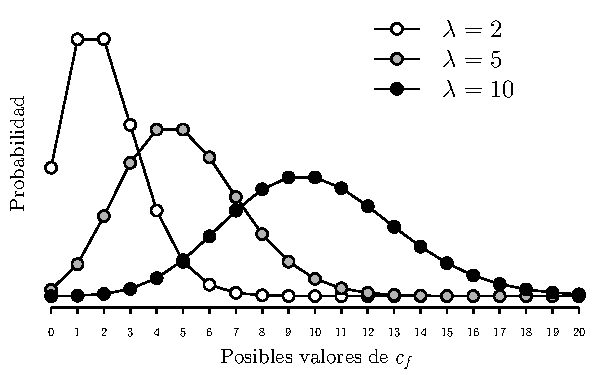
\includegraphics[trim=0cm 0cm 0cm 0cm, clip=true, width=.7\textwidth]	{poisson.pdf}
	%}
	\caption{Distribuciones Poisson para tres valores $\lambda$ diferentes.}
	\label{fig:Poisson}
	\end{figure}

\indent En otras palabras, la distribución Poisson permite calcular qué valores de $c_f$ son más probables dado un valor $\lambda$ fijo.  Podemos representar la relación probabilística entre cada posición $c_f$ y $\lambda$ con la siguiente notación:
\begin{equation}
Pr(c_f|\lambda)\sim \mathrm{Poisson}(\lambda)\label{M0_1},
\end{equation}
\noindent que se lee ``\emph{$c_f$ se distribuye Poisson con parámetro $\lambda$}''.\\
\indent Recapitulando, asumiremos que la variable aleatoria $c_f$, que representa el número de canciones que una persona baila en una fiesta, se distribuye de acuerdo con una distribución Poisson en función de $\lambda$, donde $\lambda$ representa el gusto por bailar de la persona. Llamaremos a este primer conjunto de supuestos \emph{modelo} $\mathcal M_0$.\\
\indent La idea del modelo $\mathcal M_0$, que es la idea general de cualquier modelo probabilístico, es que, incluso si el parámetro $\lambda$ es un valor fijo y estable, el número de canciones $c_f$ que la persona baila en cada fiesta es una cantidad variable. Sin embargo, la variación de $c_f$ muestra ciertas regularidades que dependen del valor $\lambda$: de acuerdo con la distribución Poisson, deberíamos esperar que una persona con un valor $\lambda$ bajo baile por lo general pocas canciones por fiesta y que una persona con un valor $\lambda$ alto baile un número de canciones elevado.\\ 
\indent\emph{Si conocemos} el valor $\lambda$ de una persona, el modelo $\mathcal M_0$ permite calcular cuántas canciones es probable que la persona baile en la siguiente fiesta. El problema es que el gusto por bailar no es una característica observable y no podemos medir su valor directamente. Sin embargo, podemos \emph{inferir} cuáles son los valores más probables de $\lambda$ utilizando las observaciones que recolectamos del individuo y la relación probabilística entre $\lambda$ y cada observación que compone al vector $c$. Este proceso de inferencia está basado en una identidad conocida como  \emph{\textbf{Regla de Bayes}} (Griffiths \& Yuille, 2006):
 
\begin{equation}
Pr(\lambda|c)=Pr(c|\lambda)Pr(\lambda)/Pr(c),
\end{equation}

\noindent en donde $Pr(\lambda|c)$ se conoce como \emph{\textbf{distribución posterior}} y especifica qué valores de $\lambda$ son más probables dado el conjunto de observaciones que hemos recolectado. De acuerdo con la Regla de Bayes, la distribución posterior depende de la función de verosimilitud, de la distribución  a priori, y de la verosimilitud marginal. La \emph{\textbf{función de verosimilitud}}, $Pr(c|\lambda)$, especifica qué tan probable es observar el vector de datos $c$ bajo cada posible valor de $\lambda$ y está completamente determinada por la ecuación \eqref{M0_1}. La \emph{\textbf{distribución a priori}}, $Pr(\lambda)$, especifica qué tan probable es cada valor del parámetro $\lambda$ antes de tomar en cuenta el vector de datos $c$ y generalmente se utiliza para expresar supuestos previos sobre cada posible valor paramétrico en el modelo bajo estudio. Finalmente, la \emph{\textbf{verosimilitud marginal}} especifica qué tan probable es observar el vector $c$ bajo todos los posibles valores del parámetro $\lambda$, y también puede calcularse a partir de la distribución principal del modelo (ecuación \eqref{M0_1}, en este primer ejemplo). \\
\indent En otras palabras, la Regla de Bayes permite calcular qué valores de $\lambda$ son más probables dado cierto conjunto fijo de datos $c$, o bien, qué deberíamos concluir sobre el gusto por bailar de la persona después de observar el número de canciones que bailó en cada fiesta del semestre. En este sentido, la Regla de Bayes es una herramienta formal que especifica cómo actualizar nuestro conocimiento a priori sobre el gusto por bailar de la persona utilizando las observaciones que recolectamos durante el semestre.\\
\indent Existen varios métodos para calcular distribuciones posteriores. En este capítulo aproximaremos las distribuciones posteriores de todos nuestros modelos utilizando un programa llamado \textbf{JAGS} (Just Another Gibbs Sampler; Plummer, 2003) y el paquete de cómputo estadístico \textbf{R} (R Core Team, 2015). Para inferir una distribución posterior con estos programas es necesario especificar los tres componentes principales del proceso de inferencia probabilística:
\begin{itemize}
\item{Un conjunto de datos. Como primer ejemplo utilizaremos el vector de observaciones $c$ con el que comenzamos el capítulo.}
\item{Un modelo que especifica la relación probabilística entre los datos y ciertos parámetros desconocidos. Como primer ejemplo utilizaremos el modelo $\mathcal M_0$, en donde $\lambda$ es el único parámetro desconocido.}
\item{Una distribución de probabilidad sobre cada parámetro desconocido del modelo. Como primer ejemplo, asumiremos que cualquier valor de $\lambda$ entre 0 y 50 es igualmente probable.}
\end{itemize}

\indent Podemos resumir estos tres componentes y las relaciones entre ellos utilizando notación gráfica (Vincent, en prensa; Lee, 2008). La Figura \ref{fig:m_0} presenta al modelo $\mathcal M_0$ escrito en esta notación: los nodos blancos representan variables o parámetros desconocidos; los grises a las variables observadas o conocidas. Las variables discretas son representadas como nodos cuadrados y las continuas como nodos circulares. Cuando un nodo tiene más de un elemento, como en el caso del vector $c$ en este ejemplo, se coloca dentro de un plato para indicar que cada elemento de dicho nodo es una replicación independiente del mismo proceso probabilístico, o bien, que el número de canciones $c_f$ que el participante bailó en cada fiesta depende de un parámetro $\lambda$ único que caracteriza a la persona. Aparte de la relación entre cada elemento $c_f$ y el nodo desconocido $\lambda$, el modelo incluye la distribución prior sobre $\lambda$, que captura los supuestos iniciales sobre este parámetro antes descritos.\\

\begin{figure}[H]
\centerline{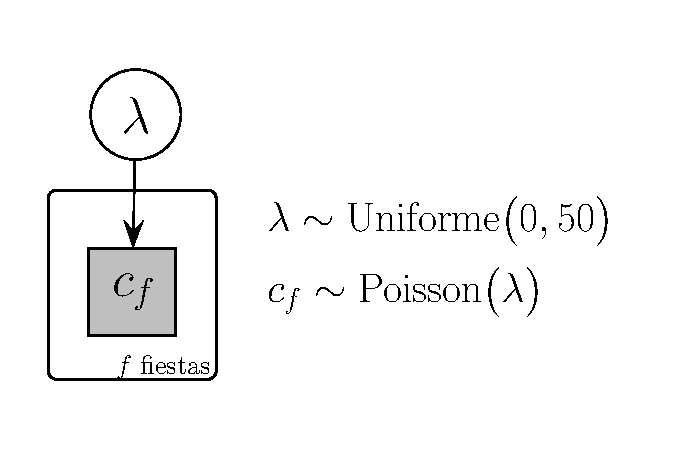
\includegraphics[width=.7\textwidth]{m_0.pdf}}
\caption{Modelo $\mathcal M_0$ expresado en notación gráfica.}
\label{fig:m_0}
\end{figure}

\indent Una vez especificado el conjunto de datos y el modelo probabilístico, el paso siguiente para hacer inferencia Bayesiana consiste en traducir el modelo gráfico a código y dejar que los programas calculen las distribuciones posteriores del modelo\footnote{Los datos y todo el código necesario para implementar los análisis de este capítulo están disponibles en: https://gist.github.com/JLBaroja/0d047481975c01c453a5}. El resultado que JAGS y R devuelven es una serie de muestreos que provienen de la distribución posterior de cada nodo desconocido en el modelo. En el caso del modelo $\mathcal M_0$, la distribución posterior sobre $\lambda$ calculada por JAGS aparece en la Figura \ref{fig:lambda_m0}. La zona gris corresponde con la densidad\footnote{Al discutir los resultados de los modelos siguientes, utilizaremos los términos \emph{distribución}, \emph{probabilidad}, y \emph{densidad} indistintamente.} posterior sobre el nodo $\lambda$, que especifica qué tan probable es cada posible valor del parámetro $\lambda$ dado el conjunto de datos $c$, de acuerdo con el modelo $\mathcal M_0$ y la Regla de Bayes. Podemos resumir cualquier distribución posterior utilizando diferentes medidas descriptivas. En la Figura \ref{fig:lambda_m0} hemos incluido la \emph{\textbf{media posterior}}, cuyo valor es igual a 5.25 y está señalada por la línea punteada, y el \emph{\textbf{intervalo de máxima densidad posterior (MDP)}} al 95\%\footnote{Presentamos el nivel de confianza = 95\% porque este valor es comúnmente empleado en inferencia estadística, aunque podemos calcular el intervalo de MDP con cualquier nivel de confianza deseado (p. ej., 90\%, 99\%).}. Este intervalo indica que podemos estar 95\% seguros de que el valor del parámetro $\lambda$ de la primera persona en observación se encuentra entre 4.02 y 6.69.

\begin{figure}[H]
\centerline{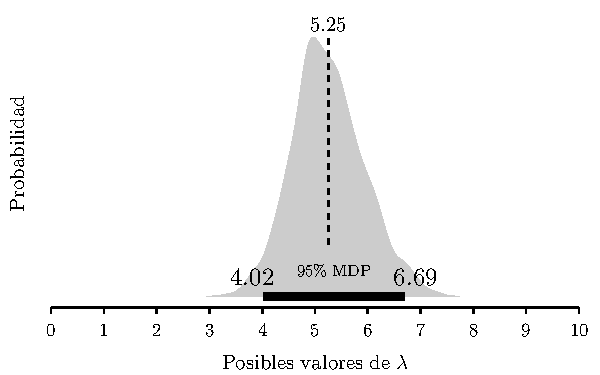
\includegraphics[width=1\textwidth]{lambda_m0.pdf}}
\caption{Distribución posterior del parámetro $\lambda$ de acuerdo con el modelo $\mathcal M_0$.}
\label{fig:lambda_m0}
\end{figure}

\indent En resumen, el modelo $\mathcal M_0$ supone que existe una variable latente $\lambda$ que refleja el gusto por bailar de una persona. De acuerdo con este modelo, existe una relación probabilística entre $\lambda$ y el número de canciones $c_f$ que la persona puede bailar en una fiesta, lo que quiere decir que aunque $\lambda$ sea una característica constante el número de canciones que la persona baila de fiesta en fiesta es una cantidad variable. Utilizando las observaciones que recolectamos a lo largo del semestre, el modelo $\mathcal M_0$, y la Regla de Bayes, calculamos los valores del gusto por bailar $\lambda$ más probables de la primera persona en nuestro estudio.\\\\
\indent Ahora extenderemos el modelo $\mathcal M_0$ para inferir el gusto por bailar de varias personas. Como estamos interesados en aprender sobre varios individuos necesitamos obtener observaciones de cada uno. La Figura \ref{fig:data} presenta la cantidad de canciones que 15 personas bailaron en las 12 primeras fiestas del semestre.\\
\indent Una inspección rápida de la Figura \ref{fig:data} sugiere que las personas son diferentes respecto al número de canciones que bailaron en cada fiesta. Los participantes 4 y 5, por ejemplo, bailaron pocas canciones en las fiestas del semestre, mientras que los sujetos 7 y 1 bailaron una cantidad de canciones elevada. Aunque cada persona bailó un número diferente de canciones en cada fiesta, la cantidad de canciones que cada persona bailó a lo largo del semestre parece relativamente estable, es decir, las personas que bailaron pocas canciones en las primeras fiestas también bailaron pocas canciones en las últimas, y quienes bailaron muchas canciones al inicio del semestre también bailaron muchas al final.\\

\begin{figure}[H]
\centering
\setlength\fboxsep{0pt}
\setlength\fboxrule{0.5pt}
%\fbox{
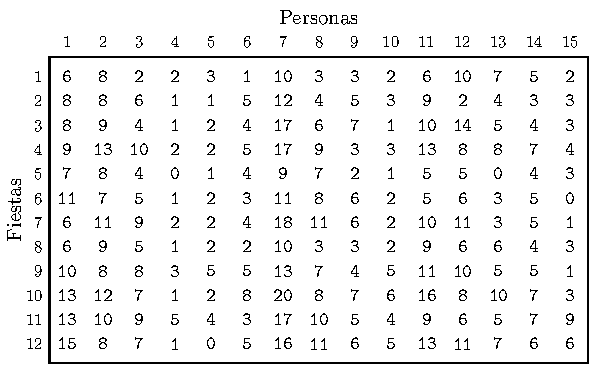
\includegraphics[trim=0cm 0cm 0cm 0cm, clip=true, width=1\textwidth]	{data_1.pdf}
%}
\caption{Conjunto de datos de todas las personas. Cada columna corresponde con una persona y cada renglón con una fiesta. Cada posición $c_{fp}$ de la matrix $c$ es el número de canciones que la persona $p$ bailó en la fiesta $f$.}
\label{fig:data}
\end{figure}

\indent Podemos extender el modelo $\mathcal M_0$ para inferir el valor del gusto por bailar de cada persona $p$, que denotamos como $\lambda_p$. La extensión simplemente consiste en suponer que cada persona tiene un valor $\lambda_p$ particular, potencialmente diferente de las demás personas. Esta extensión, a la que llamaremos $\mathcal M_1$, aparece en notación gráfica en la Figura \ref{fig:m_1}. Como puede apreciarse al examinar los modelos gráficos correspondientes, la única diferencia entre los modelos $\mathcal M_0$ y $\mathcal M_1$ es un nuevo plato que indexa personas. En otras palabras, el modelo $\mathcal M_1$ conserva la misma relación probabilística entre cada nodo $\lambda_p$ y la columna de la matriz $c$ correspondiente a la persona $p$, pero a diferencia del modelo $\mathcal M_0$, el modelo $\mathcal M_1$ supone que hay varias personas, cada una con un valor $\lambda_p$ propio.

\begin{figure}[H]
\centerline{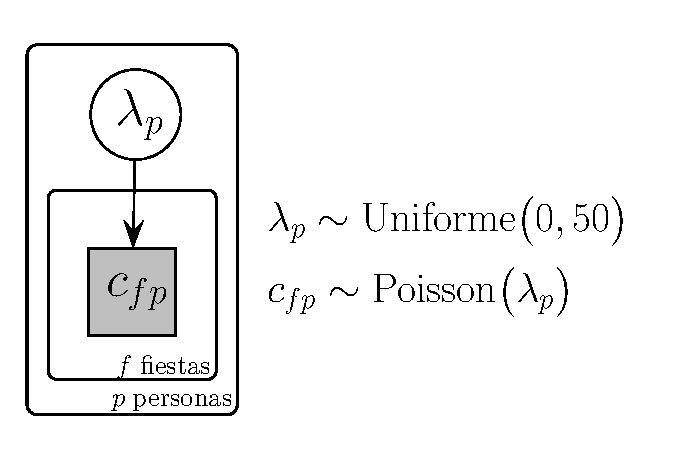
\includegraphics[width=.65\textwidth]{m_1.pdf}}
\caption{Modelo $\mathcal M_1$ expresado en notación gráfica.}
\label{fig:m_1}
\end{figure}

\indent Los resultados del modelo $\mathcal M_1$ aparecen en la Figura \ref{fig:lambda_m1}. En el panel superior de la Figura presentamos las distribuciones posteriores sobre el parámetro $\lambda_p$ de cada participante $p$. Dado que el modelo $\mathcal M_1$ asume que hay tantas personas como columnas en la matriz $c$, $\mathcal M_1$ devuelve tantas distribuciones posteriores sobre $\lambda$ como columnas en $c$. Al examinar las distribuciones posteriores sobre el nodo $\lambda_p$ podemos apreciar que el modelo $\mathcal M_1$ concluye que, aunque hay algunos participantes que se parecen entre sí, la mayoría de los participantes son diferentes respecto a su gusto por bailar, lo cual se refleja en el rango de variación de las diferentes distribuciones posteriores sobre $\lambda_p$. Al asumir que pueden existir diferencias individuales en el parámetro $\lambda_p$ el modelo $\mathcal M_1$ permite identificar a los participantes extremos P4 y P7, que resaltamos en el panel superior.\\
\indent En el panel central y en el inferior presentamos en detalle las distribuciones posteriores sobre $\lambda_p$ de los participantes 4 y 7, quienes, de acuerdo con $\mathcal M_1$, tienen el menor y el mayor gusto por bailar, respectivamente. La línea punteada en cada distribución corresponde a la media posterior, y la línea gruesa nuevamente señala el intervalo de MDP. Las conclusiones de $\mathcal M_1$ sobre los participantes 4 y 7 parecen consistentes con los datos de ambos individuos: Los participantes 4 y 7 fueron quienes bailaron menos y más canciones durante el semestre, respectivamente.\\
\indent Una forma útil de evaluar la capacidad descriptiva y predictiva de un modelo consiste en analizar la \emph{\textbf{distribución posterior predictiva}} del modelo. La distribución posterior predictiva es una distribución de probabilidad que especifica los datos que el modelo espera observar con base en los que ya han sido observados. En la Figura \ref{fig:data_1} mostramos la distribución posterior predictiva del modelo $\mathcal M_1$. El tamaño de cada círculo negro corresponde exactamente con el número de canciones que la persona $p$ bailó en la fiesta $f$ (ver Figura \ref{fig:data}). Esta representación visual permite identificar rápidamente a los participantes que bailan más, a los que bailan menos, y a los que bailan una cantidad de canciones intermedia, y también permite tener una idea clara del tamaño de las diferencias entre ellos.

\begin{figure}[H]
\centerline{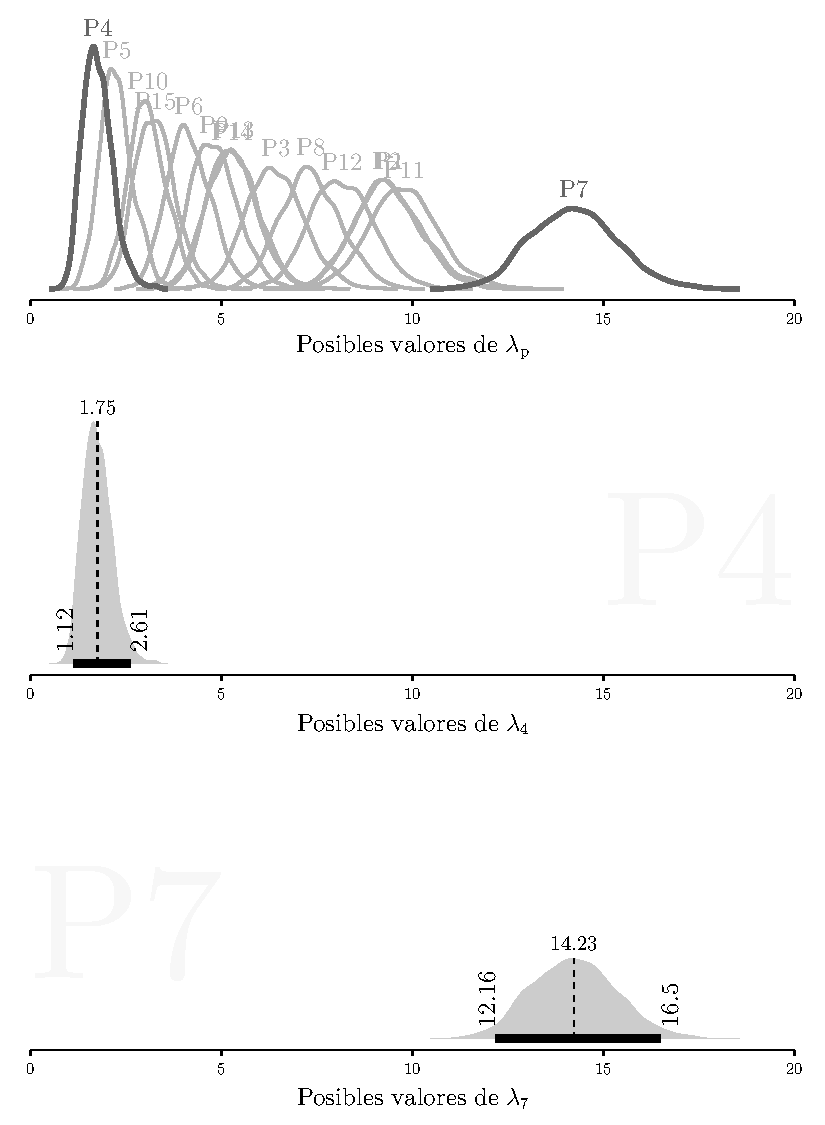
\includegraphics[width=1\textwidth]{lambda_m1.pdf}}
\caption{Distribuciones posteriores del nodo $\lambda_p$ de acuerdo con el modelo $\mathcal M_1$. Cada curva en la gráfica superior corresponde con la densidad posterior del parámetro $\lambda_p$ de cada participante. La gráfica central y la inferior detallan la distribución posterior sobre $\lambda$ de los participantes extremos (P4 y P7, respectivamente). }
\label{fig:lambda_m1}
\end{figure}

\noindent Los círculos grises en la Figura \ref{fig:data_1} señalan el intervalo de MDP de la distribución posterior predictiva de $\mathcal M_1$ sobre cada nodo $c_{fp}$.\footnote{Al implementer cualqueir modelo dentro del marco Bayesiano, el resultado es una distribución posterior sobre cada nodo del modelo. En este caso, el modelo termina con una distribución completa sobre los posibles números de canciones bailadas para cada persona $p$ en cada fiesta $f$.} Para evaluar la \emph{capacidad descriptiva} de $\mathcal M_1$ podemos comparar cada círculo negro contra el círculo gris en la posición $c_{fp}$ correspondiente. Desde la perspectiva Bayesiana, un modelo describe adecuadamente el conjunto de datos recolectados en la medida que los datos observados (círculos negros) se ubican \emph{dentro} del intervalo de MDP de la distribución posterior predictiva (círculos grises). Al comparar los datos observados contra los esperados por $\mathcal M_1$ aparecen algunas deficiencias importantes. En general, parece que algunos datos de cada participante se ubican dentro de los círculos grises mientras que otros se ubican en algún extremo. En el caso del participante 1, por ejemplo, el modelo describe adecuadamente las observaciones en las fiestas 6 y 9 porque los círculos negros se ubican en el centro de las zonas grises correspondientes. Sin embargo, $\mathcal M_1$ espera ver que el participante  1 baile más canciones que las de hecho observadas en las fiestas 7 y 8 porque los círculos negros se ubican en la frontera interior de las zonas grises, y espera ver menos que las observadas en las fiestas 10, 11 y 12 porque en estas fiestas el círculo negro se ubica en la forntera exterior de la distribución posterior predictiva. Este patrón se repite en todos los participantes: Aunque en promedio las predicciones de $\mathcal M_1$ se ajustan a las observaciones de cada persona, el modelo espera ver más canciones bailadas que las observadas en algunas fiestas, y espera ver menos canciones bailadas que las observadas en otras.\\

\begin{figure}[H]
\centering
\setlength\fboxsep{0pt}
\setlength\fboxrule{0.5pt}
%\fbox{
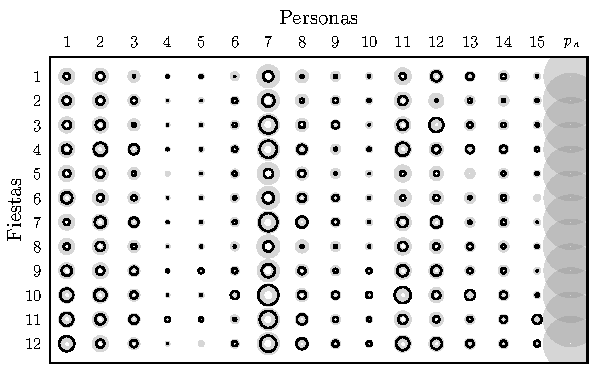
\includegraphics[trim=0cm 0cm 0cm 0cm, clip=true, width=1\textwidth]	{data_pos_pred_m1.pdf}
%}
\caption{Datos comparados contra la distribución posterior predictiva del modelo $\mathcal M_1$. Los círculos grises representan la distribución posterior predictiva del modelo y los círculos negros reflejan los datos observados. Aparte de que el ajuste entre los datos y las predicciones  $\mathcal M_1$ es cuestionable, la deficiencia principal del $\mathcal M_1$ es que no puede hacer predicciones razonables sobre cómo lucirá un participante nuevo, representado en la columna $p_n$.}
\label{fig:data_1}
\end{figure}

\indent Un problema todavía más grave del modelo $\mathcal M_1$ es su limitada \emph{capacidad predictiva}. En la Figura \ref{fig:data_1} hemos incluido una columna adicional, $p_n$, en la que presentamos los datos que el modelo $\mathcal M_1$ espera ver en un participante nuevo. Las distribuciones posteriores predictivas de dicha columna sugieren que $\mathcal M_1$ considera igualmente probable que el participante nuevo baile pocas o muchas canciones, incluso en rangos que ninguno de los participantes observados ha presentado hasta el momento. El tamaño de los círculos grises en la columna $p_n$, en relación a la escala de la figura, sugiere que el modelo considera probable que el nuevo participante hubiera bailado desde 0 hasta 30 o quizá 40 canciones en cada fiesta del semestre (ver Figura \ref{fig:data}).  ¿Por qué deberíamos esperar que un nuevo participante baile 30 o 40 canciones cuando ninguno de los observados ha bailado más de 20? $\mathcal M_1$ hace esta extraña predicción porque, aunque ha aprendido algo sobre cada participante, no ha aprendido nada sobre \emph{la población} de participantes. Como consecuencia, cuando $\mathcal M_1$ tiene que predecir cómo se comportará una persona nueva no puede utilizar el conocimiento que ha ganado sobre todas las personas que ha observado anteriormente y la predicción resulta poco informativa. Idealmente, un buen modelo debería aprender sobre cada persona y también sobre la población de personas para predecir adecuadamente cómo lucirá cada sujeto observado en las situaciones observadas e idealmente en situaciones nuevas (p. ej., la siguiente fiesta).\\\\
\indent Una posible extensión que permite aprender sobre individuos y poblaciones de individuos al mismo tiempo consiste en suponer que, aunque cada persona tiene un valor $\lambda_p$ particular, los valores $\lambda_p$ de todas las personas provienen de una población común. La notación gráfica de este nuevo modelo, denominado $\mathcal M_2$, aparece en la Figura \ref{fig:m_2}.

\begin{figure}[H]
\centerline{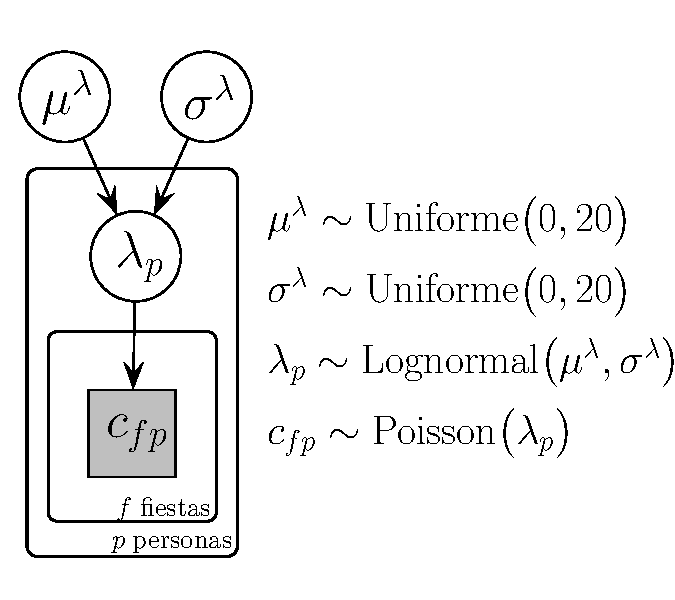
\includegraphics[width=.7\textwidth]{m_2.pdf}}
\caption{Modelo $\mathcal M_2$ expresado en notación gráfica.}
\label{fig:m_2}
\end{figure}

\indent Similar a sus predecesores, el modelo $\mathcal M_2$ conserva el supuesto central que relaciona cada nodo $\lambda_p$ con las observaciones $c_{fp}$ correspondientes, y también supone de que cada persona tiene un valor $\lambda_p$ propio. Sin embargo, $\mathcal M_2$ adicionalmente supone que todos los parámetros $\lambda_p$ provienen de una distribución poblacional común, definida por los parámetros $\mu^\lambda$ y $\sigma^\lambda$, que corresponden con la media y la desviación estándar poblacionales\footnote{Utilizamos la distribución Log-normal como distribución jerárquica porque los valores de $\lambda_p$ son mayores que cero por definición. Esta restricción vuelve inadecuado modelar la variación en $\lambda_p$ con distribuciones definidas sobre todos los números reales (p.ej., la distribución normal) (ver Limpert et al., 2001).}, respectivamente. Este supuesto adicional vuelve al modelo $\mathcal M_2$ un \emph{modelo jerárquico}.\\
\indent En general, un modelo jerárquico asume que los nodos desconocidos en cierto nivel provienen de una distribución definida en un nivel superior. Las extensiones jerárquicas pueden incluir varios niveles y, como mostraremos más adelante, pueden definirse no sólo respecto a participantes sino también respecto a estímulos o condiciones experimentales.\\
\indent La Figura \ref{fig:data_2} permite comparar los datos observados contra la distribución posterior predictiva del modelo $\mathcal M_2$. En la figura podemos observar que el ajuste de $\mathcal M_2$ es similar al ajuste de $\mathcal M_1$, es decir, ambos modelos muestran una relación similar entre los datos observados y los predichos. Sin embargo, el modelo $\mathcal M_2$ muestra mejor capacidad de predicción comparada con la del modelo $\mathcal M_1$. En particular, la predicción que $\mathcal M_2$ hace sobre un participante nuevo parece más razonable que la sugerida por el modelo anterior. $\mathcal M_2$ puede hacer una predicción sensible sobre el nuevo participante porque tiene información sobre cómo se comporta la población de participantes observados y puede usar dicha información para inferir cuál será el valor $\lambda_{p_{n}}$ de un participante nuevo.

\begin{figure}[H]
\centering
\setlength\fboxsep{0pt}
\setlength\fboxrule{0.5pt}
%\fbox{
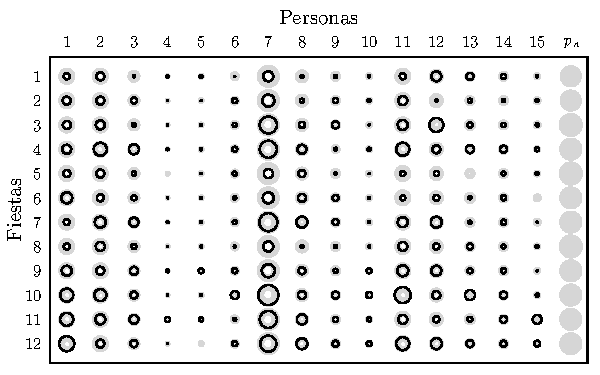
\includegraphics[trim=0cm 0cm 0cm 0cm, clip=true, width=1\textwidth]	{data_pos_pred_m2.pdf}
%}
\caption{Datos comparados contra la distribución posterior predictiva del modelo $\mathcal M_2$. La capacidad de ajuste del modelo $\mathcal M_2$ es similar a la de $\mathcal M_1$, pero el modelo $\mathcal M_2$ puede hacer predicciones informadas sobre cómo lucirá un participante nuevo.}
\label{fig:data_2}
\end{figure}

\indent También podemos examinar las conclusiones de $\mathcal M_2$ sobre el gusto por bailar de cada participante en la muestra. La Figura \ref{fig:lambda_m2} muestra estos resultados. En el panel superior nuevamente presentamos las distribuciones posteriores sobre $\lambda_p$ de cada participante. A primera vista parece que el modelo $\mathcal M_2$ concluye algo similar al modelo $\mathcal M_1$: La mayoría de los participantes tienen valores $\lambda_p$ diferentes, distribuidos aproximadamente en el mismo rango de valores bajo ambos modelos. Aparte, el modelo $\mathcal M_2$ también identifica a los participantes 4 y 7 como participantes extremos.\\
\indent Sin embargo, al estudiar en detalle las conclusiones de $\mathcal M_2$ sobre los participantes extremos aparece una diferencia muy importante entre ambos modelos. En el panel central y en el inferior presentamos las distribuciones posteriores sobre $\lambda_p$ de los participantes 4 y 7, respectivamente. En cada panel, la línea de densidad negra es la distribución posterior inferida por $\mathcal M_2$ y la gris es la densidad posterior inferida por $\mathcal M_1$ (ver Figura \ref{fig:lambda_m1}). En el caso del participante 4, el modelo $\mathcal M_2$ infiere una distribución posterior sobre valores de $\lambda_4$ mayores respecto del modelo $\mathcal M_1$: tanto la media posterior como los intervalos de la zona de MDP de $\lambda_4$ de acuerdo con $\mathcal M_2$ aparecen recorridos a la derecha respecto de los de $\mathcal M_1$. En pocas palabras, aunque el modelo $\mathcal M_2$ también concluye que  el participante 4 tiene el gusto por bailar menor en la muestra de participantes, el valor de $\lambda_4$ inferido por $\mathcal M_2$ no es tan pequeño como el inferido por $\mathcal M_1$. Algo similar ocurre en el participante 7, pero en sentido contrario: la distribución posterior sobre $\lambda_7$ calculada por $\mathcal M_2$ aparece recorrida a la izquierda con respecto a la de $\mathcal M_1$, es decir, aunque al participante 7 le gusta bailar más que al resto de la muestra, el modelo $\mathcal M_2$ concluye que el gusto por bailar de este participante no es tan grande como sugiere el modelo $\mathcal M_1$.\\
\indent Es importante resaltar que los modelos $\mathcal M_1$ y $\mathcal M_2$ llegan a conclusiones diferentes sobre los participantes extremos incluso cuando ambos modelos observaron \emph{exactamente} los mismos datos de cada participante. Si ambos modelos observan los mismos datos de cada participante, ¿por qué llegan a conclusiones diferentes? La razón es que en el modelo $\mathcal M_1$ la única información relevante para inferir cada nodo $\lambda_p$ son las observaciones del participante correspondiente, mientras que bajo el modelo $\mathcal M_2$ los valores $\lambda_p$ inferidos en cada participante dependen de las observaciones del participante y también de las observaciones de todos los participantes en la muestra. Cuando $\mathcal M_2$ calcula el gusto por bailar del participante 4, por ejemplo, concluye algo como: \emph{las observaciones de P4 sugieren que este participante tiene un gusto por bailar pequeño, pero dado que el participante proviene de una población de individuos que tienen un gusto por bailar intermedio, debería creer que su gusto por bailar no es tan pequeño después de todo}, y algo similar ocurre respecto al participante 7 en la dirección opuesta. En general, en cualquier modelo jerárquico las conclusiones sobre cada sujeto, cada ítem o cada condición experimental dependen no sólo de las observaciones de cada elemento sino también de las observaciones de la población correspondiente. Este efecto es una característica importante de los modelos jerárquicos y se conoce como \emph{\textbf{contracción jerárquica}} (Rouder et al., 2017). \\

\begin{figure}[H]\centerline{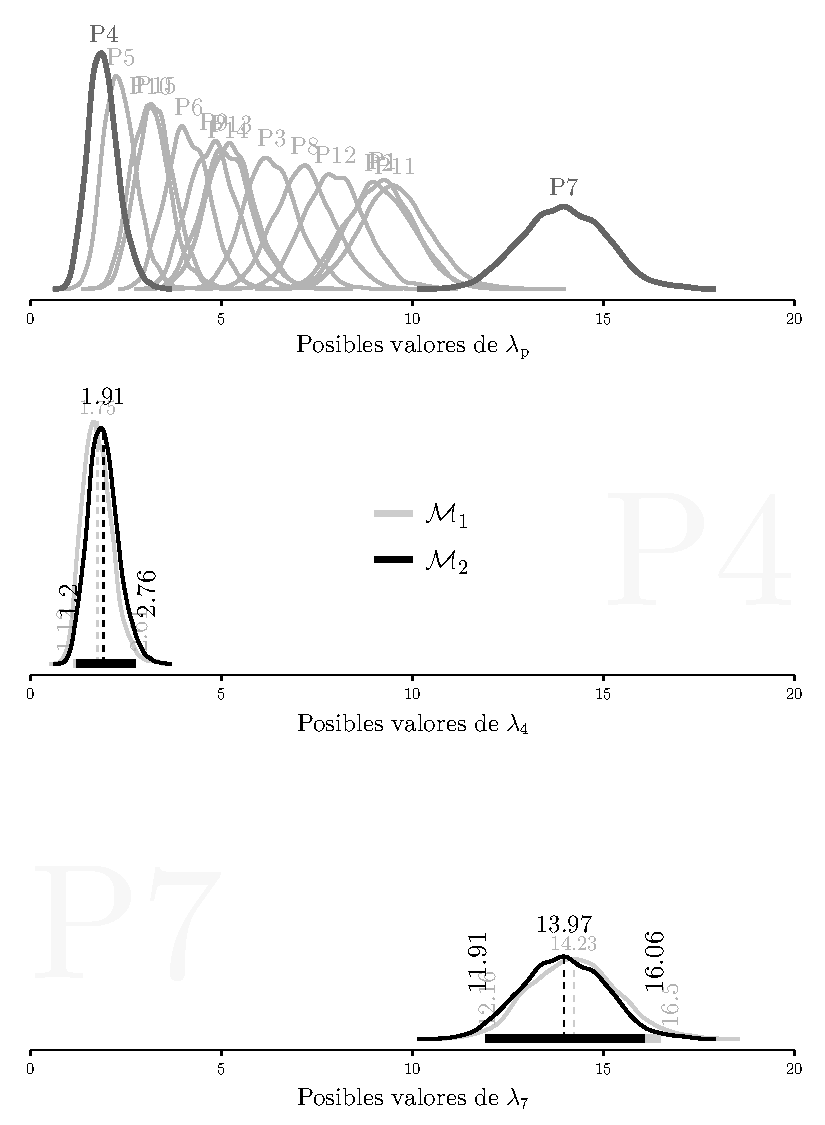
\includegraphics[width=1\textwidth]{lambda_m2.pdf}}
\caption{Distribuciones posteriores del nodo $\lambda_p$ de acuerdo con el modelo $\mathcal M_2$. Aunque el modelo $\mathcal M_2$ observa \emph{exactamente} los mismos datos que el modelo $\mathcal M_1$, $\mathcal M_2$ llega a conclusiones diferentes sobre los participantes extremos: En el modelo $\mathcal M_2$ las distribuciones posteriores sobre $\lambda$ de los participantes 4 y 7 no son tan extremas como en el modelo $\mathcal M_1$.}
\label{fig:lambda_m2}
\end{figure}

\indent En el modelo $\mathcal M_2$ los parámetros $\mu^\lambda$ y $\sigma^\lambda$ corresponden con la media y la desviación estándar de la distribución poblacional de \emph{gustos por bailar}, que suponemos son diferentes para cada persona. Podemos examinar las distribuciones posteriores sobre ambos parámetros para averiguar qué valores son más probables en cada uno. La Figura \ref{fig:hierarchical_lambda_m2} presenta las distribuciones posteriores sobre los parámetros poblacionales inferidas por el modelo $\mathcal M_2$.

\begin{figure}[H]
\centerline{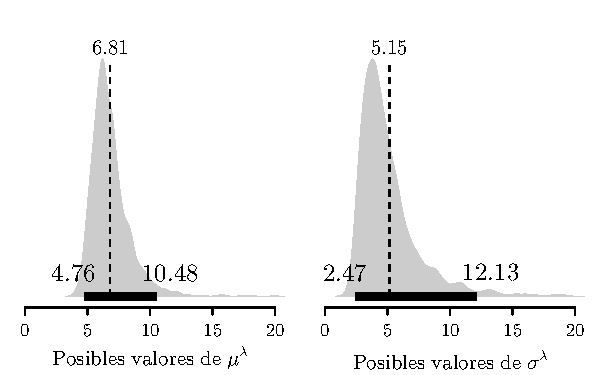
\includegraphics[width=.8\textwidth]{hierarchical_lambda_m2.pdf}}
\caption{Distribuciones posteriores de los parámetros $\mu^\lambda$ y $\sigma^\lambda$ poblacionales de acuerdo con el modelo $\mathcal M_2$.}
\label{fig:hierarchical_lambda_m2}
\end{figure}

\indent Recapitulando, el modelo $\mathcal M_2$ asume que las variables latentes $\lambda_p$, que corresponden con el gusto por bailar de cada persona en la población, provienen de la misma distribución poblacional. Este supuesto permite a $\mathcal M_2$ inferir los valores paramétricos poblacionales y utilizar dichos valores para predecir cómo hubiera lucido un nuevo participante si hubiéramos registrado el número de canciones que bailó en cada fiesta del semestre. La capacidad de predecir a un nuevo participante es una ventaja importante de $\mathcal M_2$ respecto de su antecesor.\\
\indent Sin embargo, tanto $\mathcal M_1$ como $\mathcal M_2$ comparten una deficiencia descriptiva más sutil. En concreto, aunque las predicciones de los dos modelos se acercan a los datos observados en cada participante, en algunas fiestas ambos modelos esperan que los participantes bailen más canciones que las que de hecho bailaron (p.ej., en la fiesta 5), mientras que en otras los dos modelos esperan ver que los participantes bailen menos de lo que bailaron (p.ej., fiesta 10; ver Figuras \ref{fig:data_1} y \ref{fig:data_2}). En las secciones siguientes sugerimos cómo mejorar estas deficiencias.\\\\
\indent Los modelos que hemos construido y evaluado hasta el momento comparten un supuesto central: Suponen que la cantidad de canciones que cada persona bailó en cada fiesta sólo depende del gusto por bailar de la persona. Aunque este supuesto es razonable parece incompleto, como lo sugiere una inspección detallada de ciertas tendencias en los datos observados. En particular, parece que hay fiestas en las que todas las personas tienden a bailar más canciones. La fiesta 7 y la 4 son ejemplos de este tipo de fiestas. Por el contrario, en otras fiestas la mayoría de la muestra de participantes bailó pocas canciones, como en la fiesta 8 o en la 5. Estos patrones sugieren que la cantidad de canciones que una persona baila en una fiesta no sólo depende del gusto por bailar de la persona sino también de alguna característica \emph{de la fiesta}, como el número de canciones que tocaron en ella. Si en una fiesta tocan pocas canciones esperamos observar que una persona baile pocas canciones incluso si tiene un gusto por bailar alto; o bien, si en una fiesta tocan muchas canciones esperamos observar que personas a las que les gusta bailar poco bailen más canciones que de costumbre.\\
\indent Los modelos que presentamos a continuación formalizan estas intuiciones y las ponen a prueba.\\\\
\indent El modelo $\mathcal M_3$, que aparece en notación gráfica en la Figura \ref{fig:m_3}, supone que la cantidad de canciones que la persona $p$ bailó en la fiesta $f$, $c_{fp}$, depende del gusto por bailar de la persona, esta vez anotado como $\theta_p$, y del número de canciones que tocaron en la fiesta, $n_f$.

\begin{figure}[H]
\centerline{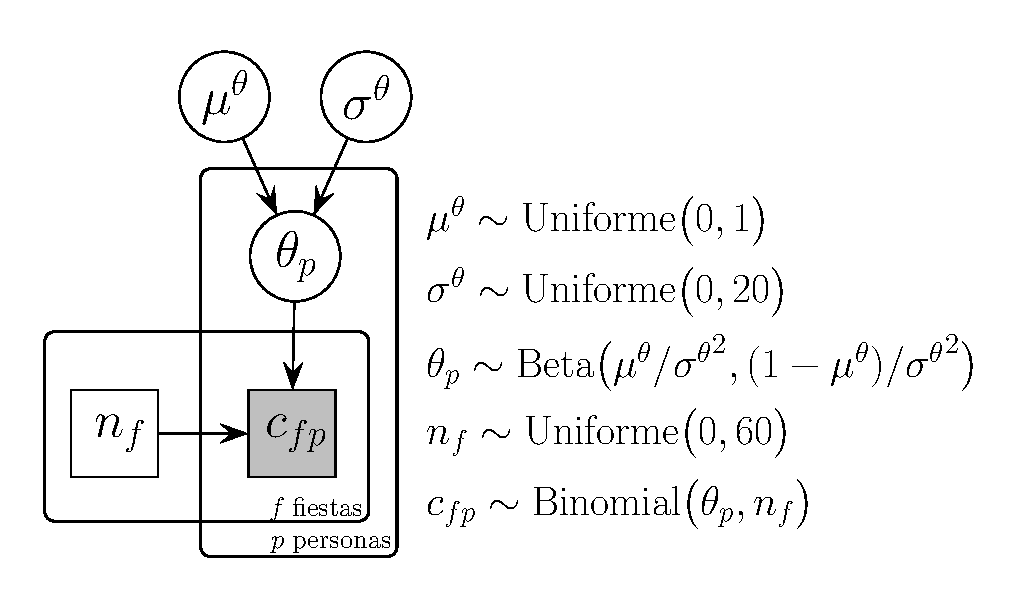
\includegraphics[width=1\textwidth]{m_3.pdf}}
\caption{Modelo $\mathcal M_3$ expresado en notación gráfica.}
\label{fig:m_3}
\end{figure}

\indent Es importante destacar que tanto el gusto por bailar de la persona $\theta_p$ como el número de canciones que tocaron en cada fiesta, $n_f$, son nodos no observados que afectan condicionalmente a la variable observada $c_{fp}$, y por lo tanto podemos inferir el valor de ambos parámetros desconocidos utilizando el mismo conjunto de herramientas de inferencia que hemos presentado previamente. Como el parámetro $\theta_p$ es una característica de la persona que suponemos se mantiene constante entre fiestas, el nodo $\theta_p$ aparece indexado en el plato de personas pero fuera del plato de fiestas. Por su parte, el nodo $n_f$ está dentro del plato de fiestas pero fuera del plato de personas para reflejar el supuesto de que la cantidad de canciones que tocaron en la fiesta $f$ es una característica propia de cada fiesta.\\
\indent De acuerdo con $\mathcal M_3$ la cantidad de canciones que la persona $p$ bailó en la fiesta $f$ es una variable aleatoria con distribución Binomial con parámetros $\theta_p$ y $n_f$:

\begin{equation}
Pr(c_{fp}|\theta_p,n_f)\sim \mathrm{Binomial}(\theta_p,n_f)\label{M3_1},
\end{equation}

\indent Elegimos la distribución Binomial porque esta distribución tiene dos propiedades que parecen reflejar el escenario de las fiestas. Primero, entre más grande es el parámetro $n$ en una distribución Binomial el valor esperado de la variable aleatoria aumenta, al margen del valor del parámetro $\theta$. Segundo, entre más grande es el valor del parámetro $\theta$ el valor esperado de la variable aleatoria también aumenta, al margen del valor de $n$. En tanto que el parámetro $\theta$ en una distribución Binomial está restringido al rango $0\leq\theta\leq1$ necesitamos especificar una distribución jerárquica que esté definida para variables aleatorias en dicho rango. La distribución Beta cumple con esta característica. Como hemos hecho explícito en el modelo gráfico, en $\mathcal M_3$ parametrizamos la distribución Beta en términos de la media $\mu^\theta$ y desviación estándar $\sigma^\theta$ de la población de \emph{personas}. Utilizamos distribuciones prior uniformes sobre los nodos del modelo $\mathcal M_3$; en el caso de los nodos $n_f$ y $\sigma^\theta$ los límites de la distribución prior fueron elegidos arbitrariamente, pero en el caso del nodo $\mu^\theta$ el rango de valores válidos está restringido por la distribución que depende de dicho nodo: como la distribución Beta está definida únicamente dentro del intervalo (0,1), los valores de la media de dicha distribución también tienen que ubicarse en el mismo intervalo.\\ 
\indent Los resultados del modelo $\mathcal M_3$ se resumen en la Figura \ref{fig:data_3}. Al comparar la distribución posterior predictiva de $\mathcal M_3$ contra los datos registrados observamos que esta vez los círculos negros se ubican en medio de las zonas grises con mayor frecuencia, lo cual indica que en la mayoría de los casos la predicción de $\mathcal M_3$ se acerca a las observaciones recolectadas de cada persona. Aparte, $\mathcal M_3$ también parece predecir adecuadamente cómo se comportará un participante nuevo. $\mathcal M_3$ predice sensiblemente a un nuevo participante porque conserva la estructura jerárquica sobre participantes del modelo $\mathcal M_2$. Es decir, incluso si cambiamos la distribución jerárquica específica (de Log-normal a Beta, en este ejemplo), el hecho de suponer que todos los participantes provienen de una distribución poblacional común es suficiente para predecir el desempeño de un participante nuevo utilizando el conocimiento adquirido al observar a la muestra de personas.\\
\indent En la misma Figura hemos incluido un renglón adicional que representa la siguiente fiesta del semestre, que tendrá lugar la semana entrante. Un buen modelo sobre el fenómeno bajo estudio debería predecir no sólo cómo se comportará un participante nuevo en las fiestas conocidas, sino también cómo se comportarán los participantes conocidos en una fiesta nueva.\\
\indent Al examinar la distribución posterior predictiva de $\mathcal M_3$ en la fiesta nueva aparecen conclusiones sospechosas. En concreto, aunque $\mathcal M_3$ predice que las personas que han bailado más canciones en las fiestas observadas también bailarán más en la fiesta nueva, la cantidad de canciones que $\mathcal M_3$ espera ver en la fiesta nueva parece poco informada. En el caso del participante 7, por ejemplo, $\mathcal M_3$ espera ver que este participante baile cualquier número de canciones entre 0 y 25, aproximadamente. ¿Por qué esperarías que un participante que consistentemente ha bailado más de 9 canciones en las fiestas del semestre baile 1 o 2 en la fiesta siguiente? O bien, ¿por qué este participante bailaría hasta 25 canciones, si en ninguna fiesta ha bailado más de 20?\\

\begin{figure}[H]
\centering
\setlength\fboxsep{0pt}
\setlength\fboxrule{0.5pt}
%\fbox{
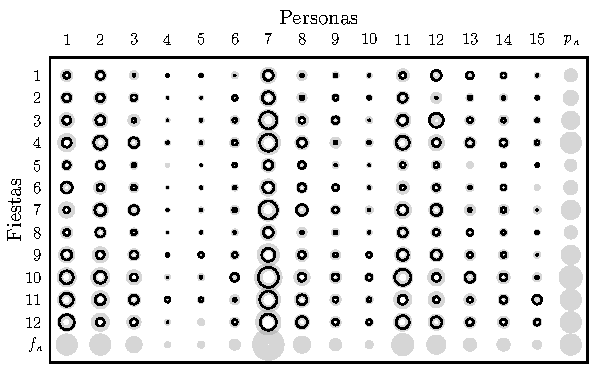
\includegraphics[trim=0cm 0cm 0cm 0cm, clip=true, width=1\textwidth]	{data_pos_pred_m3.pdf}
%}
\caption{Datos comparados contra la distribución posterior predictiva del modelo $\mathcal M_3$. Aunque $\mathcal M_3$ hace predicciones razonables sobre un participante nuevo la predicción sobre una fiesta nueva parece poco informada.}
\label{fig:data_3}
\end{figure}
	
\indent Si planteamos estas preguntas a $\mathcal M_3$ podemos adivinar su respuesta: \emph{aunque he aprendido sobre el participante 7 y sobre la población de la que este participante proviene, no puedo hacer buenas predicciones sobre cuánto bailará este participante en la siguiente fiesta porque no sé cuántas canciones tocarán en ella}. En otras palabras, aunque $\mathcal M_3$ infiere cuántas canciones tocaron en cada fiesta \emph{observada}, no puede utilizar dicho conocimiento para predecir una fiesta nueva. Para utilizar el conocimiento ganado sobre las fiestas observadas y predecir adecuadamente cuántas canciones tocarán en la siguiente fiesta es conveniente suponer que todas las fiestas tienen algo en común, o bien, que provienen de la misma distribución jerárquica.\\
	
\indent El modelo $\mathcal M_4$, que presentamos en la Figura \ref{fig:m_4}, es una extensión del modelo $\mathcal M_3$ que adicionalmente supone que la cantidad de canciones que tocaron en cada fiesta, $n_f$, proviene de una distribución de fiestas jerárquica. \\

\begin{figure}[H]
\centerline{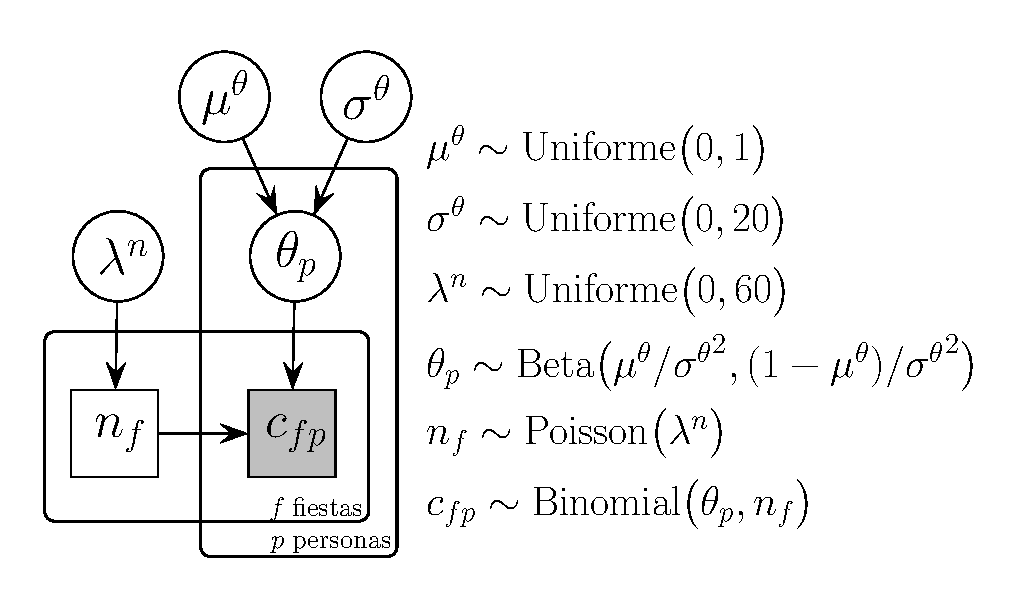
\includegraphics[width=1\textwidth]{m_4.pdf}}
\caption{Modelo $\mathcal M_4$ expresado en notación gráfica.}
\label{fig:m_4}
\end{figure}

\begin{figure}[H]
\centering
\setlength\fboxsep{0pt}
\setlength\fboxrule{0.5pt}
%\fbox{
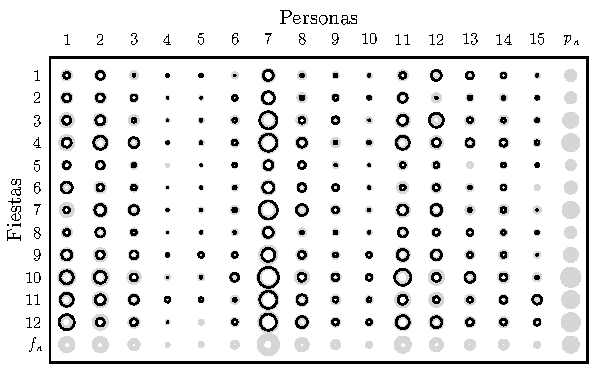
\includegraphics[trim=0cm 0cm 0cm 0cm, clip=true, width=1\textwidth]	{data_pos_pred_m4.pdf}
%}
\caption{Datos comparados contra la distribución posterior predictiva del modelo $\mathcal M_4$. Al suponer una distribución jerárquica sobre participante y otra sobre fiestas, este modelo puede hacer predicciones sensibles sobre cómo lucirá un participante nuevo y una fiesta nueva.}
\label{fig:data_4}
\end{figure}
	
\indent	Cuando el modelo $\mathcal M_4$ observa los datos que recolectamos infiere cuántas canciones tocaron en cada fiesta, de manera similar a $\mathcal M_3$, pero $\mathcal M_4$ también infiere el valor del parámetro $\lambda_n$, que representa la media y la varianza de la distribución poblacional de fiestas. En consecuencia, $\mathcal M_4$ puede utilizar este conocimiento para predecir cuántas canciones tocarán en la fiesta siguiente (y por lo tanto cuántas de ellas bailará cada persona). Como resultado, las predicciones de $\mathcal M_4$ sobre cómo lucirá una fiesta nueva, que presentamos en la Figura \ref{fig:data_4}, parecen mucho más razonables que las de $\mathcal M_3$.\\
\indent Resumiendo, el suponer una distribución jerárquica sobre participantes y una distribución jerárquica sobre fiestas permite al modelo $\mathcal M_4$ predecir cuánto hubiera bailado un participante nuevo en cada fiesta conocida, cuánto bailarán los participantes conocidos en una fiesta nueva, y cuánto bailará un participante nuevo en una fiesta nueva. \\\\
\indent En este capítulo hemos desarrollado diferentes modelos que sirven para inferir características individuales y poblacionales con base en cierto conjunto de datos. Las extensiones jerárquicas respecto a personas y respecto a fiestas mejoran el ajuste y la capacidad predictiva de nuestros modelos, o bien, de nuestras explicaciones sobre el mundo.\\
\indent Los modelos Bayesianos jerárquicos son una poderosa herramienta de inferencia que tiene un rango enorme de aplicación en psicología: Lo único necesario para implementarlos es contar con un modelo que especifique una relación probabilística entre cierto rasgo psicológico y cierto conjunto de observaciones. Por ejemplo, si suponemos que la probabilidad de recordar un ítem depende de qué tan buena es la memoria de una persona y de qué tan difícil es recordar el ítem, podemos inferir la \emph{capacidad de retención} personal y la \emph{dificultad del memorización} del ítem si pedimos a la persona que memorice el ítem y después registramos si lo memorizó o no. En caso de registrar el desempeño de varios participantes en la tarea, cada uno recordando varios ítems que potencialmente difieren en dificultad, es pertinente asumir que todos los participantes provienen de una población común respecto del rasgo \emph{capacidad de retención} y que todos los ítems provienen de su propia distribución jerárquica respecto de la \emph{dificultad de memorización}. El suponer distribuciones jerárquicas sobre participantes y sobre ítems permite computar estimaciones más precisas sobre ambos rasgos, como lo sugieren algunos resultados reportados por Jeff Rouder y colaboradores (Rouder y Lu, 2005; Rouder et al., 2007). 

\section*{Lecturas recomendadas}
	\begin{itemize}
	
	\item[]{Lee, M. D. (2008). Three case studies in the Bayesian analysis of cognitive models. \emph{Psychonomic Bulletin \& Review, 15,} 1-15.}

	\item[]{Lee, M. D., \& Wagenmakers, E.-J. (2014). \emph{Bayesian Cognitive Modeling: A Practical Course.} Cambridge University Press.}
	
    \item[]{Rouder, J. N., Morey, R. D. \& Pratte, M. S. (2017). Bayesian hierarchical models of cognition. En W. H. Batchelder, H. Colonius, E. Dzhafarov, y J. I. Myung, (Eds.), \emph{The New Handbook of Mathematical Psychology, Volume 1: Measurement and Methodology.} Cambridge University Press.} 
    
     \item[]{Shiffrin, R. M., Lee, M. D., Kim, W. \& Wagenmakers, E.-J. (2008). A survey of model evaluation approaches with a tutorial on hierarchical Bayesian methods. \emph{Cognitive Science, 32,} 1248-1284.}
      
    \end{itemize}


    
\section*{Referencias}
	\begin{itemize}
	\setlength{\itemindent}{-.15in}
	
%	\item[]{Bertsekas, D. P. \& Tsitsiklis, J. N. (2008). \emph{Introduction to Probability (2nd ed.).} MIT Press.}
	
	\item[]{Griffiths, T. L. \& Yuille, A. (2006). Technical introduction: A primer on probabilistic inference. http://dx.doi.org/doi:10.1016/j.tics.2006.05.007}
	
	\item[]{Limpert, E., Stahel, W. A. \& Abbt, M. (2001). Log-normal distributions across the sciences: Keys and clues. \emph{BioScience, 51,} 341-352.}
	
    \item[]{Plummer, M. (2003). JAGS: A program for analysis of Bayesian graphical models using Gibbs sampling. \emph{Proceedings of the 3rd International Workshop on Distributed Statistical Computing,} 20-22.}
    
    \item[]{R Core Team (2015). R: A language and environment for statistical
  computing. R Foundation for Statistical Computing, Vienna, Austria. URL
  http://www.R-project.org/.}
  
    \item[]{Rouder, J. N. \& Lu, J. (2005). An introduction to Bayesian hierarchical models with an application in the theory of signal detection. \emph{Psychonomic Bulletin \& Review, 12,} 573-604.}
    
    \item[]{Rouder, J. N., Lu, J., Sun, D., Speckman, P. L., Morey, R. D. \& Naveh-Benjamin, M. (2007). Signal detection models with random participant and item effects. \emph{Psychometrika, 72,} 621-642.}
     
    \item[]{Vincent, B. T. (en prensa). A tutorial on Bayesian models of perception. \emph{Journal of Mathematical Psychology.}         doi:10.1016/j.jmp.2015.02.001}
     
    \end{itemize}
    
    




\end{document}